\section{Slab configuration Drawing}\label{slab-configuration-drawing}

The slab configuration used in the slab model is a ``slab in grade'' model. That is, the slab top surface is assumed level with the outside earth surface. If a ``slab on grade'' configuration, having the bottom surface of the slab level with the outside earth surface is desired, the best approximation is to use the horizontal insulation configuration. The edge of the slab will have a small thermal resistance due to the two dimensional path through the earth, but the effect is small. In any case, uninsulated slab edges are certainly not recommended in cold climates.

\begin{figure}[hbtp] % fig 20
\centering
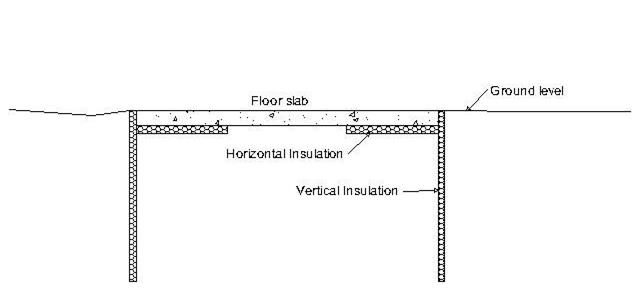
\includegraphics[width=0.9\textwidth, height=0.9\textheight, keepaspectratio=true]{media/image018.jpg}
\caption{Slab-in-grade illustration \protect \label{fig:slab-in-grade-illustration}}
\end{figure}
